\documentclass [9 pt]{article}
\usepackage[margin = 1in]{geometry}
\usepackage{amsfonts}
\usepackage{amsthm}
\usepackage{bbm}
 \usepackage{amsmath}
\usepackage[utf8]{inputenc}
\usepackage{graphicx}
\usepackage{ wasysym }
\usepackage{enumerate}
\usepackage{color}
\usepackage{graphicx}
\graphicspath{ {./images/} }
\usepackage{tikz}
\usepackage{booktabs}

\theoremstyle{definition}
\newtheorem{problem}{Problem}
\newtheorem{theorem}{Theorem}
\newtheorem*{corollary}{Corollary}
\newtheorem{proposition}[theorem]{Proposition}
\newtheorem{lemma}[theorem]{Lemma}
\newtheorem{conjecture}[theorem]{Conjecture}

\newtheorem{definition}[theorem]{Definition}
\newtheorem{remark}[theorem]{Remark}
\newtheorem{example}[theorem]{Example}


\usepackage{fancyhdr}
\pagestyle{fancy}
\lhead{Yuhao Wu \quad 260711365} 
\rhead{\bfseries COMP 330 Assignment 2}
\cfoot{\thepage}
\renewcommand{\headrulewidth}{0.4pt}
\renewcommand{\footrulewidth}{0.4pt}





\begin{document}

\title{COMP 330 Assignment 2}
\date{2018-9-24}
\author{Name: Yuhao Wu\\
ID Number: 260711365
}
\maketitle


\section*{Question 1:}
Give regular expressions for the following languages over $\{a, b\}$:
\begin{itemize}
	\item  $\{w|w \text{ contains an even number of occurrences of } a\}$
	\item $\{w|w \text{ contains an odd number of occurrences of } b\}$
	\item $\{w|w \text{ does not contain the substring } ab\}$
	\item $\{w|w \text{ does not contain the substring } aba\}$
\end{itemize}
\textbf{SOLUTION:} \\
(1):$$\bigg( b^* a b^* a \bigg)^*b^* $$
(2):$$ \bigg( a^*ba^*b \bigg)^* a^* b a^* $$
(3): "b" can be followed by any letter but "a" can be only followed by "a"
$$b^* a^*$$
(4): "a" may be followed by either  "a" or by "bb"\\
But when I am ending, I can have "a" followed by "b" as there is no more letters coming
$$ b^* \bigg(a^*bb\quad b^*\bigg)^* a^* b^*$$











\newpage
\section*{Question 2:}
Suppose that you have a DFA $M = (S,\Sigma,s_0,\delta,F)$ . Consider two distinct states $s_1$,$s_2$ i.e. $s_1 \neq s_2$. Suppose further that for all $a \in \Sigma, \delta(s_1,a) = \delta(s_2,a)$. Show that for any nonempty word $w$ over $\Sigma$ we have  $\delta^{*}  (s_1,w) = \delta^{*} (s_2, w)$.
\begin{proof}
	We prove by induction on the length of word $|w|$
	\begin{itemize}
		\item Base Case: we start with word with length 1, which means $|w| = 1$\\
		Obviously, we have that $$\delta^*(s_1,a) = \delta(s_1,a) = \delta(s_2,a) = \delta^*(s_2,a).$$
		\item Inductive Step: Suppose it is true for word $x$, which means that 
		$$ \delta^{*}  (s_1,x) = \delta^{*} (s_2, x) $$
		Then for $w = x a$, we have
		\begin{align*}
			\delta^{*}  (s_1,xa) 
			&= \delta\bigg( \delta^{*}  (s_1,x), a \bigg)\\
			&= \delta\bigg( \delta^{*}  (s_2,x), a \bigg) \textbf{ By induction hypothesis} \\
			&=  \delta^{*}  (s_2,xa )\\
		\end{align*}
	\end{itemize}
\end{proof}








\newpage
\section*{Question 3:}
Show that the following languages are not regular by using the pumping lemma.
\begin{itemize}
	\item 1. $L = \{a^nb^ma^{n+m}|n, m \geq 0\}$,
 	\item 2. $L = \{x|x = x^R, x \in \Sigma^*\}$ , where $x^R$ means x reversed; these strings are called palindromes. An example is $abba$, a non-example is $baba$.
\end{itemize}


\subsection*{(a):}
\begin{itemize}
	\item Demon pick a random variable $p$ \\
	
	
	\item I pick $w = a^pb^1a^{p+1}$, obviously $w \in L$ and $ |w| \geq p$\\


	\item Then Demon needs to pick $x, y, z$ such that $w = xyz$ and $|xy| \leq p, |y| > 0$ \\
	\newline
	As $|xy| \leq p$, Demon's $y$ must contain "a" only, which means $y = a^k \quad 0 < k \leq p$ \\
	
	
	
	\item I will choose $i = 2$, such that $xy^2z = a^{p +  k}b^1 a^{p+1} $\\\\
	Obviously, $p + k + 1 > p + 0 + 1 = p + 1$\\\\
	Thus $xy^2z \notin L $.\\
	\newline
	\textbf{ Therefore, the language is not regular. }
\end{itemize}


\subsection*{(b):}
\begin{itemize}
	\item Demon pick a random variable $p$\\
	
	\item I pick $w = a^pba^{p}$, obviously $w \in L$ and $ |w| \geq p$ \\
	
	\item Then Demon needs to pick $x, y, z$ such that $w = xyz$ and $|xy| \leq p, |y| > 0 $ \\\\
	As $|xy| \leq p$, Demon's $y$ must contain "a" only, which means that $ y = a^k \quad 0 <  k \leq p$\\
	\item I will choose $i = 2$, such that $xy^2z = a^{p +  k}b a^{p} $\\\\
	Obviously, $p + k > p + 0 =  p $, so $w = xy^2z $ can't be palindrome\\\\
	Thus $xy^2z \notin L $\\
	\newline
	\textbf{ Therefore, the language is not regular. }
\end{itemize}







\newpage
\section*{Question 4:}
Show that the following languages are not regular by using the pumping lemma.
\begin{itemize}
	\item(a) $L = \{x \in \{a, b, c\}^*||x| \text{ is a square.} \}$ Here $|x|$ means the length of $x$
	\item(b) $L = \{a^{2n}b^n\}$
\end{itemize}

\subsection*{(a):}
\begin{itemize}
	\item Demon pick a random value $p$
	\item I pick $w = a^{p^2}$, so $|w| = p^2$ and obviously $|w| \geq p$ 
	\item Then Demon needs to pick $x, y, z$ such that $w = xyz$ and $|xy| \leq p, |y| > 0 $ \\\\
	 Suppose that: $ y = a^k \quad 0 <  k \leq p$\\
	\item I will choose $i = 2$, such that $ xy^2z = a^{p^2 + k} $, so we have $|xy^2z | = p^2 + k$\\
	we have:
	\begin{align*}
		|xy^2z | &= p^2 + k \\
		& \leq p^2 + p \\
		&< (p+1)^2
	\end{align*}
	And we have $|xy^2z | = p^2 + k > p^2 + 0 = p^2$, \\
	Thus, we have $ p^2 < |xy^2z | < (p+1)^2 $ so we can say that $|xy^2z |$ is not a square $\implies xy^2z \notin L$.\\
	\newline
		\textbf{ Therefore, the language is not regular. }
\end{itemize}

\subsection*{(b):}
\begin{itemize}
	\item Demon pick a random value $p$ \\
	
	\item I pick $w = a^{2p}b^p$ obviously $|w| > p$ and $w \in L$ \\
	
	\item Then Demon needs to pick $x, y, z$ such that $w = xyz$ and $|xy| \leq p, |y| < 0$ \\\\
	As $|xy| \leq p$, Demon's $y$ must contain "a" only, which is  $ y  = a^{k}\text{ with } 0 < k \leq p$ \\
	
	
	\item I will choose $i = 2$, such that $xy^2z = a^{2p +  k}b^{p} $\\ \\
	$$ \dfrac{2p+k}{p} = 2 + \dfrac{k}{p} > 2 \implies xy^2z \notin L $$
	\newline
	\textbf{ Therefore, the language is not regular. }
\end{itemize}

\newpage
\section*{Question 5:}
We are using the alphabet $\{0,1\}$. We have a DFA with 5 states, $S = \{s_0, s_1, s_2, s_3, s_4\}$. The start state is $s_0$ and the only accepting state is also $s_0$. The transitions are given by the formula
$$\delta(s_i,a) = s_j\textbf{ Where  }  j=i^2+a\quad mod 5$$
Draw the table showing which pairs of states are inequivalent and then construct the minimal automaton. Remember to remove useless states right from the start, before you draw the table. I am happy with a drawing of the automaton.
\\ \newline \newline \newline\newline
$$\delta(s_0,0) = s_0 \quad \delta(s_0,1) = s_1  \quad \delta(s_1,0) = s_1  \quad \delta(s_1,1) = s_2     $$
$$\delta(s_2,0) = s_4 \quad \delta(s_2,1) = s_0  \quad \delta(s_3,0) = s_4  \quad \delta(s_3,1) = s_0    $$
 $$\delta(s_4,0) = s_1  \quad \delta(s_4,1) = s_2     $$



\begin{center}
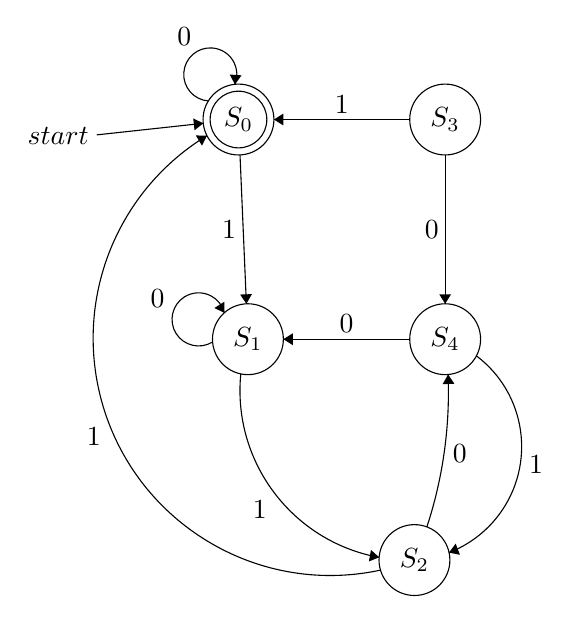
\begin{tikzpicture}[scale=0.15]
\tikzstyle{every node}+=[inner sep=0pt]
\draw [black] (21.3,-13.2) circle (3);
\draw (21.3,-13.2) node {$S_0$};
\draw [black] (21.3,-13.2) circle (2.4);
\draw [black] (22.1,-31.8) circle (3);
\draw (22.1,-31.8) node {$S_1$};
\draw [black] (36.2,-50.5) circle (3);
\draw (36.2,-50.5) node {$S_2$};
\draw [black] (38.8,-31.8) circle (3);
\draw (38.8,-31.8) node {$S_4$};
\draw [black] (38.8,-13.2) circle (3);
\draw (38.8,-13.2) node {$S_3$};
\draw [black] (9.3,-14.5) -- (18.32,-13.52);
\draw (8.65,-14.6) node [left] {$start$};
\fill [black] (18.32,-13.52) -- (17.47,-13.11) -- (17.58,-14.11);
\draw [black] (18.758,-11.629) arc (266.00538:-21.99462:2.25);
\draw (16.72,-6.98) node [above] {$0$};
\fill [black] (21,-10.23) -- (21.56,-9.46) -- (20.56,-9.39);
\draw [black] (21.43,-16.2) -- (21.97,-28.8);
\fill [black] (21.97,-28.8) -- (22.44,-27.98) -- (21.44,-28.02);
\draw (21.14,-22.52) node [left] {$1$};
\draw [black] (19.12,-32.028) arc (302.11719:14.11719:2.25);
\draw (15.09,-28.4) node [left] {$0$};
\fill [black] (20.11,-29.57) -- (20.1,-28.63) -- (19.26,-29.16);
\draw [black] (33.214,-50.274) arc (-100.32139:-185.64524:14.36);
\fill [black] (33.21,-50.27) -- (32.52,-49.64) -- (32.34,-50.62);
\draw (23.74,-46.19) node [left] {$1$};
\draw [black] (39.046,-34.789) arc (2.34537:-18.1764:36.564);
\fill [black] (39.05,-34.79) -- (38.58,-35.61) -- (39.58,-35.57);
\draw (39.41,-41.48) node [right] {$0$};
\draw [black] (33.326,-51.35) arc (-77.79509:-238.65507:20.086);
\fill [black] (18.63,-14.56) -- (17.69,-14.55) -- (18.21,-15.41);
\draw (9.68,-40.05) node [left] {$1$};
\draw [black] (35.8,-13.2) -- (24.3,-13.2);
\fill [black] (24.3,-13.2) -- (25.1,-13.7) -- (25.1,-12.7);
\draw (30.05,-12.7) node [above] {$1$};
\draw [black] (38.8,-16.2) -- (38.8,-28.8);
\fill [black] (38.8,-28.8) -- (39.3,-28) -- (38.3,-28);
\draw (38.3,-22.5) node [left] {$0$};
\draw [black] (41.438,-33.204) arc (53.04764:-68.87867:9.622);
\fill [black] (39.12,-49.87) -- (40.05,-50.05) -- (39.69,-49.11);
\draw (45.87,-42.38) node [right] {$1$};
\draw [black] (35.8,-31.8) -- (25.1,-31.8);
\fill [black] (25.1,-31.8) -- (25.9,-32.3) -- (25.9,-31.3);
\draw (30.45,-31.3) node [above] {$0$};
\end{tikzpicture}
\end{center}

As we can see from the above automata, $S_3$ is unreachable. So, when we build the table without $S_3$
\newpage
\textbf{First Step:} $S_0$ is accept state and $S_1, S_2, S_4$ are reject states, so we set position $(0,1), (0,2), (0,4)$ as 0
\newline
\newline
\begin{center}

\begin{tabular}{ c|ccc  c} 
\specialrule{0em}{5pt}{5pt}

$S_4$  & \quad & \quad & \quad & $\times$      \\


$S_2$  & \quad & \quad & $\times$   \\

$S_1$  & \quad & $\times$     \\
 
$S_0$  &$\times$  &0 & 0 &0          \\
  \hline 
&$S_0$ & $S_1$ & $S_2$ & $S_4$ \\


\end{tabular}
\end{center}




\textbf{Second Step:}
\begin{itemize}
	\item $\bigg(\delta(S_1, 1),  \delta(S_2, 1) \bigg) \implies (S_2, S_0) $
	\item  $\bigg(\delta(S_1, 1),  \delta(S_3, 1) \bigg) \implies (S_2, S_0) $  
	\item 	$\bigg(\delta(S_2, 1),  \delta(S_4, 1) \bigg) \implies (S_0, S_2) $  
\end{itemize}
\begin{center}
\begin{tabular}{ c|ccc  c} 
\specialrule{0em}{5pt}{5pt}

$S_4$  & \quad & \quad & \quad  & $\times$      \\


$S_2$  & \quad & \quad & $\times$   & 0  \\

$S_1$  & \quad & $\times$ & 0 &     \\
 
$S_0$  &$\times$  &0 & 0  &0          \\
  \hline 
&$S_0$ & $S_1$ & $S_2$  & $S_4$ \\


\end{tabular}
\end{center}

\textbf{Third Step:} we set the remaining position as 1
\begin{center}
\begin{tabular}{ c|ccc  c} 
\specialrule{0em}{5pt}{5pt}

$S_4$  & \quad & \quad & \quad  & $\times$      \\

$S_2$  & \quad & \quad & $\times$ & 0  \\

$S_1$  & \quad & $\times$ & 0 &1   \\
 
$S_0$  &$\times$  &0 & 0 & 0        \\
  \hline 
&$S_0$ & $S_1$ & $S_2$  & $S_4$ \\


\end{tabular}
\end{center}

Thus, we can say that 
$$\begin{cases}
S_1 \text{ is equivalent to } S_4\\
 S_3 \text{ is unreachable state and has been removed}\\	
\end{cases}$$

\textbf{FINAL RESULT:}
\begin{center}
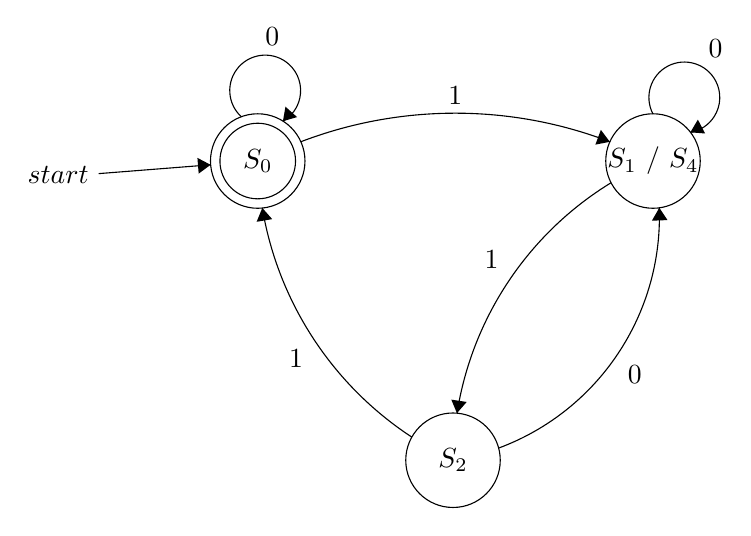
\begin{tikzpicture}[scale=0.2]
\tikzstyle{every node}+=[inner sep=0pt]
\draw [black] (26.1,-19.6) circle (3);
\draw (26.1,-19.6) node {$S_0$};
\draw [black] (26.1,-19.6) circle (2.4);
\draw [black] (38.5,-38.6) circle (3);
\draw (38.5,-38.6) node {$S_2 $};
\draw [black] (51.2,-19.6) circle (3);
\draw (51.2,-19.6) node {$S_1\mbox{ }/\mbox{ }S_4$};
\draw [black] (25.067,-16.796) arc (227.96106:-60.03894:2.25);
\draw (27.02,-12.3) node [above] {$0$};
\fill [black] (27.7,-17.07) -- (28.6,-16.81) -- (27.86,-16.15);
\draw [black] (16,-20.4) -- (23.11,-19.84);
\draw (15.39,-20.46) node [left] {$start$};
\fill [black] (23.11,-19.84) -- (22.27,-19.4) -- (22.35,-20.4);
\draw [black] (35.886,-37.133) arc (-123.25326:-170.48727:21.684);
\fill [black] (26.39,-22.58) -- (26.03,-23.46) -- (27.02,-23.29);
\draw (29,-32.17) node [left] {$1$};
\draw [black] (51.596,-22.569) arc (2.10394:-69.62315:15.666);
\fill [black] (51.6,-22.57) -- (51.13,-23.39) -- (52.12,-23.35);
\draw (49.57,-33.19) node [right] {$0$};
\draw [black] (28.837,-18.376) arc (110.95427:69.04573:27.438);
\fill [black] (48.46,-18.38) -- (47.89,-17.62) -- (47.54,-18.56);
\draw (38.65,-16.06) node [above] {$1$};
\draw [black] (38.755,-35.613) arc (171.03159:121.44921:20.992);
\fill [black] (38.75,-35.61) -- (39.37,-34.9) -- (38.39,-34.75);
\draw (41.43,-25.88) node [left] {$1$};
\draw [black] (51.199,-16.612) arc (207.75405:-80.24595:2.25);
\draw (55.17,-13.04) node [above] {$0$};
\fill [black] (53.57,-17.78) -- (54.51,-17.85) -- (54.05,-16.97);
\end{tikzpicture}
\end{center}



\end{document}